\documentclass[11pt,a4paper]{article}
\usepackage[utf8]{inputenc}
\usepackage[T1]{fontenc}
\usepackage[spanish,es-noshorthands]{babel}
\usepackage{lmodern}
\usepackage[margin=2.3cm]{geometry}
\usepackage{amsmath,amssymb}
\usepackage{booktabs,array,graphicx,xcolor}
\usepackage[colorlinks=true,linkcolor=blue!50!black,urlcolor=blue!50!black]{hyperref}
\usepackage{enumitem}
\setlist{itemsep=2pt,topsep=4pt}
\newcommand{\lt}{\tilde{\ell}}
\newcommand{\obs}[1]{\par\smallskip\noindent\colorbox{orange!12}{\parbox{\dimexpr\linewidth-2\fboxsep}{\small #1}}\par\smallskip}

\title{\textbf{Fase 1: modelo teórico del electrón de Lee--Wick}\\[3pt]
\large Reproducción de Sánchez, ACI \textbf{15}(1) 2780 (2023)}
\author{Proyecto \texttt{lw-cms-opendata}}
\date{18 de octubre de 2026}

\begin{document}
\maketitle

\begin{abstract}
\noindent Se implementó desde cero el electrón de Lee--Wick $\lt$ en FeynRules como extensión de \texttt{SM.fr}, se exportó el UFO y se calculó el ancho $\Gamma(\lt\to Ze)$ por tres vías independientes: analítica (Python), FeynRules (\texttt{ComputeWidths}) y MadGraph5 (\texttt{compute\_widths}). Las tres coinciden entre sí (MG5/FR $=1\pm4\times10^{-5}$) y reproducen la longitud de vuelo $\lambda$ de la Tabla~1 del paper con precisión $10^{-6}$ para $M_{\lt}=200$--$500$~GeV, \textbf{siempre que se use $m_e=0.5$~MeV} en el acoplamiento de mezcla. Se identificaron dos erratas en la Ec.~1 del paper (signo del término de mezcla y carga del $\lt_R$ bajo el $Z$) y se dejaron como parámetros conmutables del modelo. El trabajo se repartió entre dos agentes en paralelo (modelo y validación) y se cruzó al final.
\end{abstract}

\section{Organización del trabajo}
\begin{center}
\small
\begin{tabular}{>{\raggedright\arraybackslash}p{3.2cm}>{\raggedright\arraybackslash}p{6.0cm}>{\raggedright\arraybackslash}p{5.4cm}}
\toprule
Agente & Tarea & Productos\\
\midrule
Modelo & FeynRules (copia parcheada para Mathematica 15), comprobaciones, UFO, anchos con FR y MG5~3.8.1 & \texttt{model/LWElectron.fr}, \texttt{run\_fr.wls}, \texttt{LWElectron\_UFO/}, \texttt{mg5\_widths.py}, \texttt{widths.csv}, \texttt{README.md}, \texttt{logs/}\\
Validación & Ancho analítico, esquemas electrodébiles, revisión de Alvarez et al.\ (0908.2446) y del LWSM (0704.1845) & \texttt{validation/width\_analytic.py}, \texttt{widths\_schemes.csv}, \texttt{ctau\_vs\_M.png}, \texttt{README.md}\\
\bottomrule
\end{tabular}
\end{center}
Los hallazgos del agente de validación (valor de $m_e$, hermiticidad, representación del $\lt$) se le pasaron al agente del modelo mientras trabajaba, y se incorporaron al modelo final.

\section{El modelo}
\begin{itemize}
\item \textbf{Partícula nueva:} \texttt{elw-}/\texttt{elw+}, PDG 9000011, Dirac, $Q=-1$, masa \texttt{MLW} (200~GeV por defecto) y ancho \texttt{WLW}.
\item \textbf{Lagrangiano:} el sector NC de la Ec.~1 más el acoplamiento al fotón, necesario para la producción $q\bar q\to\gamma^*/Z^*\to\lt^+\lt^-$. El único canal de desintegración es la mezcla $e$--$\lt$--$Z$, con acoplamiento
\[
g_{\rm mix}=(g_Z^{e_L}-g_Z^{e_R})\,\frac{m_e}{M_{\lt}}=-\frac{g}{2c_W}\,\frac{m_e}{M_{\lt}},\qquad \mathrm{BR}(\lt\to Ze)=1 .
\]
\item \textbf{Parámetros nuevos} (bloque \texttt{LWINPUTS}):
  \begin{itemize}
  \item \texttt{MeLW}: el $m_e$ de la mezcla, $5.0\times10^{-4}$~GeV por defecto.
  \item \texttt{etaLW}: el signo LW de los vértices $\lt\lt\gamma$ y $\lt\lt Z$, $-1$ por defecto.
  \item \texttt{lwRep}: cómo se acopla $\lt_R$ al $Z$: $0$ = Ec.~1 literal ($g_R$); $1$ = compañero de un doblete vectorial ($g_L$), como en Alvarez et al.
  \end{itemize}
\item \textbf{Comprobaciones superadas:}
  \begin{itemize}
  \item prueba de cordura del SM (se encuentra el vértice $ee\gamma$, sin corrupción \texttt{crea});
  \item \texttt{CheckHermiticity} del lagrangiano completo: sin vértices, es decir, hermítico;
  \item normalización cinética y espectro de masas;
  \item el UFO se importa en MG5 sin errores;
  \item \texttt{ComputeWidths} de FeynRules coincide simbólicamente con la fórmula analítica (diferencia 0).
  \end{itemize}
\end{itemize}

\section{Resultado: ancho y longitud de vuelo}
En el esquema $G_F$ (que coincide con los valores por defecto de \texttt{SM.fr}: $\alpha^{-1}=127.9$, $G_F$, $m_Z=91.1876$) el ancho no depende de $s_W$:
\begin{equation}
\Gamma(\lt\to Ze)=\frac{G_F\,m_e^2\,M_{\lt}}{16\sqrt2\,\pi}\,(1-x)^2(1+2x),\qquad x=\frac{m_Z^2}{M_{\lt}^2},\qquad c\tau_0=\frac{\hbar c}{\Gamma}.
\end{equation}
El factor $M^3/m_Z^2$ procede del $Z$ longitudinal. Para $M\gg m_Z$ el resultado tiende a $y_e^2M/64\pi$, como exige la equivalencia con los Goldstone.

\begin{table}[h]
\centering\footnotesize\setlength{\tabcolsep}{4pt}
\begin{tabular}{c|ccc|c|cc}
\toprule
 & \multicolumn{3}{c|}{$m_e=0.5$ MeV} & & \multicolumn{2}{c}{$m_e=0.511$ MeV}\\
$M_{\lt}$ (GeV) & $\Gamma_{\rm FR}$ (GeV) & $c\tau_0^{\rm FR}$ (mm) & $c\tau_0^{\rm MG5}$ (mm) & $\lambda_{\rm paper}$ (mm) & $c\tau_0^{\rm FR}$ (mm) & cociente\\
\midrule
200 & $7.28775\times10^{-12}$ & $2.70765\times10^{-2}$ & $2.70767\times10^{-2}$ & $2.70765\times10^{-2}$ & $2.59234\times10^{-2}$ & 0.95741\\
300 & $1.20102\times10^{-11}$ & $1.64300\times10^{-2}$ & $1.64302\times10^{-2}$ & $1.64300\times10^{-2}$ & $1.57303\times10^{-2}$ & 0.95741\\
400 & $1.62795\times10^{-11}$ & $1.21212\times10^{-2}$ & $1.21208\times10^{-2}$ & $1.21212\times10^{-2}$ & $1.16050\times10^{-2}$ & 0.95741\\
500 & $2.04432\times10^{-11}$ & $9.65243\times10^{-3}$ & $9.65255\times10^{-3}$ & $9.65243\times10^{-3}$ & $9.24134\times10^{-3}$ & 0.95741\\
\bottomrule
\end{tabular}
\caption{Con $m_e=0.5$~MeV, $c\tau_0^{\rm FR}/\lambda_{\rm paper}=1.000000\pm1.4\times10^{-6}$. Con el valor del PDG el cociente es constante y vale $(0.5/0.511)^2=0.9574$.}
\end{table}

\begin{figure}[h]
\centering
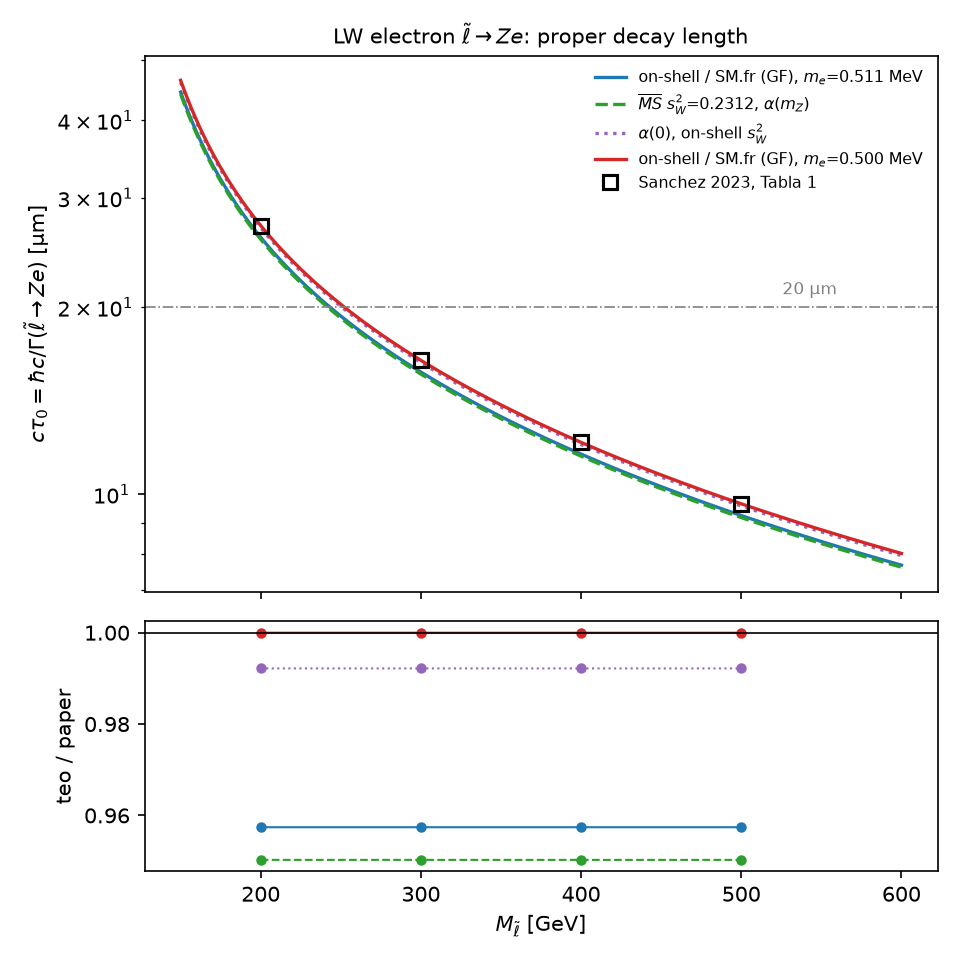
\includegraphics[width=0.62\linewidth]{../validation/ctau_vs_M.png}
\caption{$c\tau_0$ frente a $M_{\lt}$ para varios esquemas electrodébiles y dos valores de $m_e$, comparado con la Tabla~1. Sólo la curva roja ($G_F$, $m_e=0.5$~MeV) pasa por los cuatro puntos. El esquema $\overline{\rm MS}$ da $0.950$, y $\alpha(0)$ da $0.992$.}
\end{figure}

\textbf{Conclusiones:}
\begin{enumerate}
\item El $\lambda$ del paper es la longitud de desintegración \emph{propia} $c\tau_0$, sin boost, y sólo cuenta el canal $Ze$.
\item El autor usó $m_e=0.5$~MeV y el esquema electrodébil por defecto de FeynRules. Es una elección redondeada, pero hay que conservarla para reproducir su Tabla~1.
\item El modelo queda validado para la desintegración, que fija la geometría de los vértices desplazados.
\end{enumerate}

\section{Erratas y decisiones de modelado}
\obs{\textbf{1. Hermiticidad.} El término de mezcla de la Ec.~1, $\bar e_R\gamma^\mu\lt_R-\bar\lt_R\gamma^\mu e_R$, es antihermítico con un coeficiente real, y FeynRules lo confirma con vértices $\pm2i\,g_{\rm mix}$. La diagonalización de la Ec.~A2 de Alvarez et al.\ da el signo ``$+$''. El modelo usa la forma hermítica; $|\mathcal{M}|^2$ de la desintegración no cambia.}
\obs{\textbf{2. Carga del $\lt_R$ bajo el $Z$.} La Ec.~1 le asigna $-g_R$, que es la carga del singlete. En Alvarez et al.\ (Ec.~B1, Ec.~7) y en el LWSM (0704.1845, Ec.~54) el $\lt$ es el compañero del doblete y $\lt_R$ lleva $-g_L$. El ancho no cambia, pero $\sigma(pp\to\lt\lt)$ podría cambiar en un factor $\sim0.5$--$0.6$ según una estimación partónica. Queda conmutable con \texttt{lwRep}; la fase~2 decidirá cuál reproduce $\sigma=5.97$~fb.}
\obs{\textbf{3. Signo LW (\texttt{etaLW}).} El UFO tiene propagadores de norma positiva; la naturaleza acausal no está en el propagador, sino que se impondrá en la geometría del vértice. En la producción de pares hay un único vértice $\lt\lt V$, así que $\eta=\pm1$ es una fase global sin efecto. Pero en procesos con dos vértices sobre la misma línea $\lt$ (radiación de un fotón desde $\lt$, correcciones de orden superior) sólo $\eta=+1$ es consistente con la invariancia gauge en un UFO de norma positiva. \textbf{Recomendación:} usar \texttt{etaLW = +1} en la generación de la fase~2.}
\obs{\textbf{4. Canales omitidos.} En el LWSM completo existe $\lt\to he$, con $\Gamma(he)\to\Gamma(Ze)$ a masas grandes, de modo que $\mathrm{BR}(Ze)\approx0.71,\,0.59,\,0.55,\,0.53$ para $M=200$--$500$~GeV. $\lt\to W\nu$ está suprimido por un factor $m_e/M$ adicional. El paper toma $\mathrm{BR}(Ze)=1$, y el modelo lo sigue para reproducirlo; es una sobreestimación de la señal a señalar en la extensión.}
\obs{\textbf{5. Convención de signo del $Z$.} \texttt{SM.fr} tiene el signo global del $Z$ opuesto al de la Ec.~1. Se mapeó con $Z\to-Z$, que invierte todos los acoplamientos del $Z$ a la vez y conserva los signos relativos.}

\section{Avance para la fase 2}
La literatura (Alvarez et al., Ec.~1, que remite a Grinstein--O'Connell--Wise 0805.2156) confirma la prescripción para la señal acausal: el vértice secundario aparece en la dirección \emph{opuesta} al momento visible, con la misma ley exponencial de longitud $\beta\gamma c\tau_0$. Hay dos formas de implementarlo: generar la desintegración causal y reflejar el desplazamiento, o invertir $\kappa_\parallel$ como el paper.

Una estimación sin PDFs (a verificar con MG5) da $\langle\beta\gamma_T\rangle\approx0.4$--$0.55$, es decir $\langle L_T\rangle\approx11$--$14~\mu$m para $M=200$~GeV. Sólo un 15--22\% de las desintegraciones superaría los $20~\mu$m de resolución, lo que anticipa una eficiencia de señal baja.

\textbf{Pendientes para la fase 2:}
\begin{enumerate}
\item Calcular $\sigma(pp\to\lt^+\lt^-)$ a 8~TeV con \texttt{lwRep}=0 y 1, compararla con la Tabla~1 y fijar \texttt{lwRep} y el PDF.
\item Generar con \texttt{time\_of\_flight} y la reflexión del vértice, y obtener la distribución real de $L_T$.
\end{enumerate}

\vspace{6pt}
\noindent\textbf{Cómo repetirlo:} \texttt{wolframscript -file model/run\_fr.wls}; \texttt{python3 model/mg5\_widths.py}; \texttt{python3 -I validation/width\_analytic.py}. Los detalles están en los \texttt{README.md} de cada carpeta.
\end{document}
